% Biographies moved out of the submission-length build during Pass 2.

\begin{IEEEbiography}[{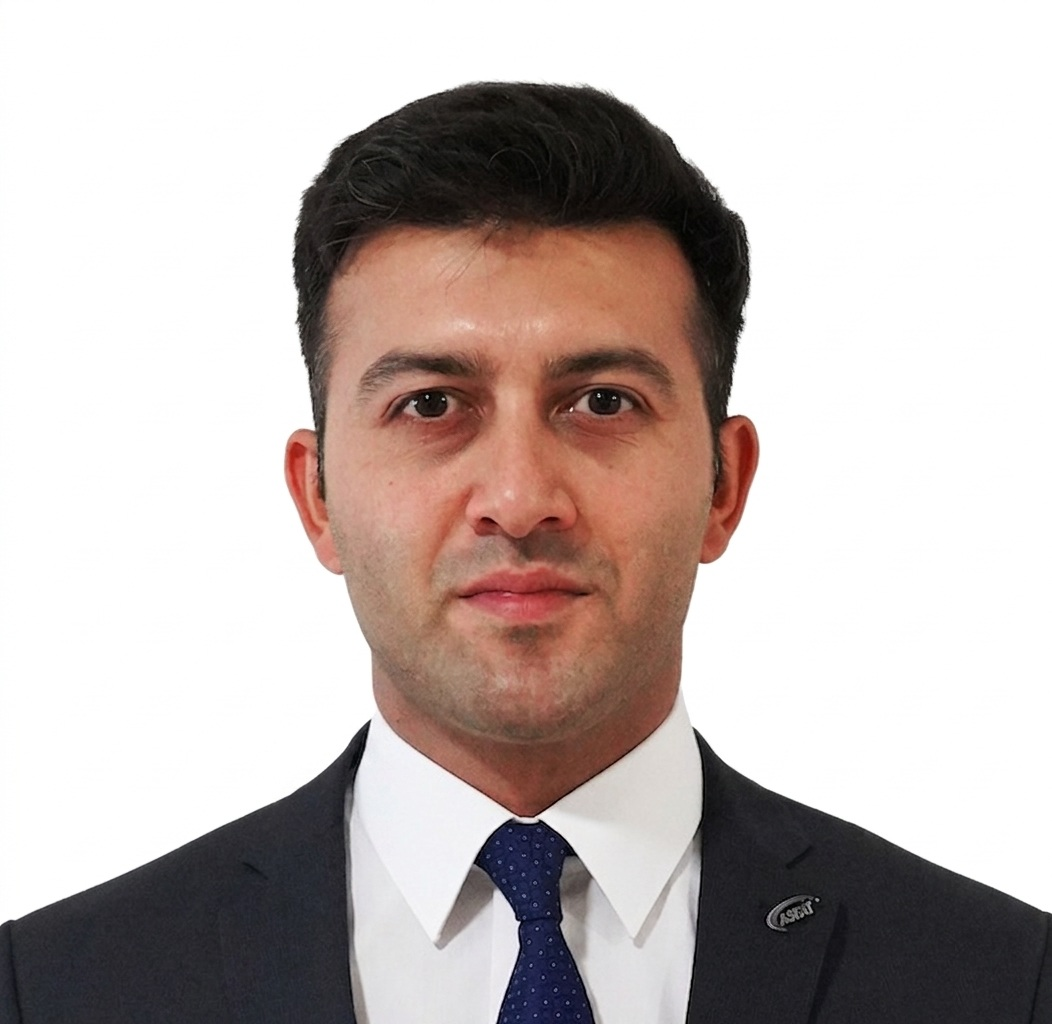
\includegraphics[width=1in,height=1.25in,clip,keepaspectratio]{figures/foto_fatih.jpg}}]{Fatih D\"onmez}
    received the B.S. degree in electrical and electronics engineering from TOBB University of Economics and Technology, Ankara, Turkiye, in 2012, and the M.S. degree in electrical and electronics engineering from Kutahya Dumlupinar University, Kutahya, Turkiye, in 2022. He is currently pursuing the Ph.D. degree in electrical and electronics engineering with Afyon Kocatepe University, Afyonkarahisar, Turkiye. His research interests include communication networks, wireless communications, communication system optimization, and integrated sensing and communication (ISAC).
\end{IEEEbiography}

\begin{IEEEbiography}[{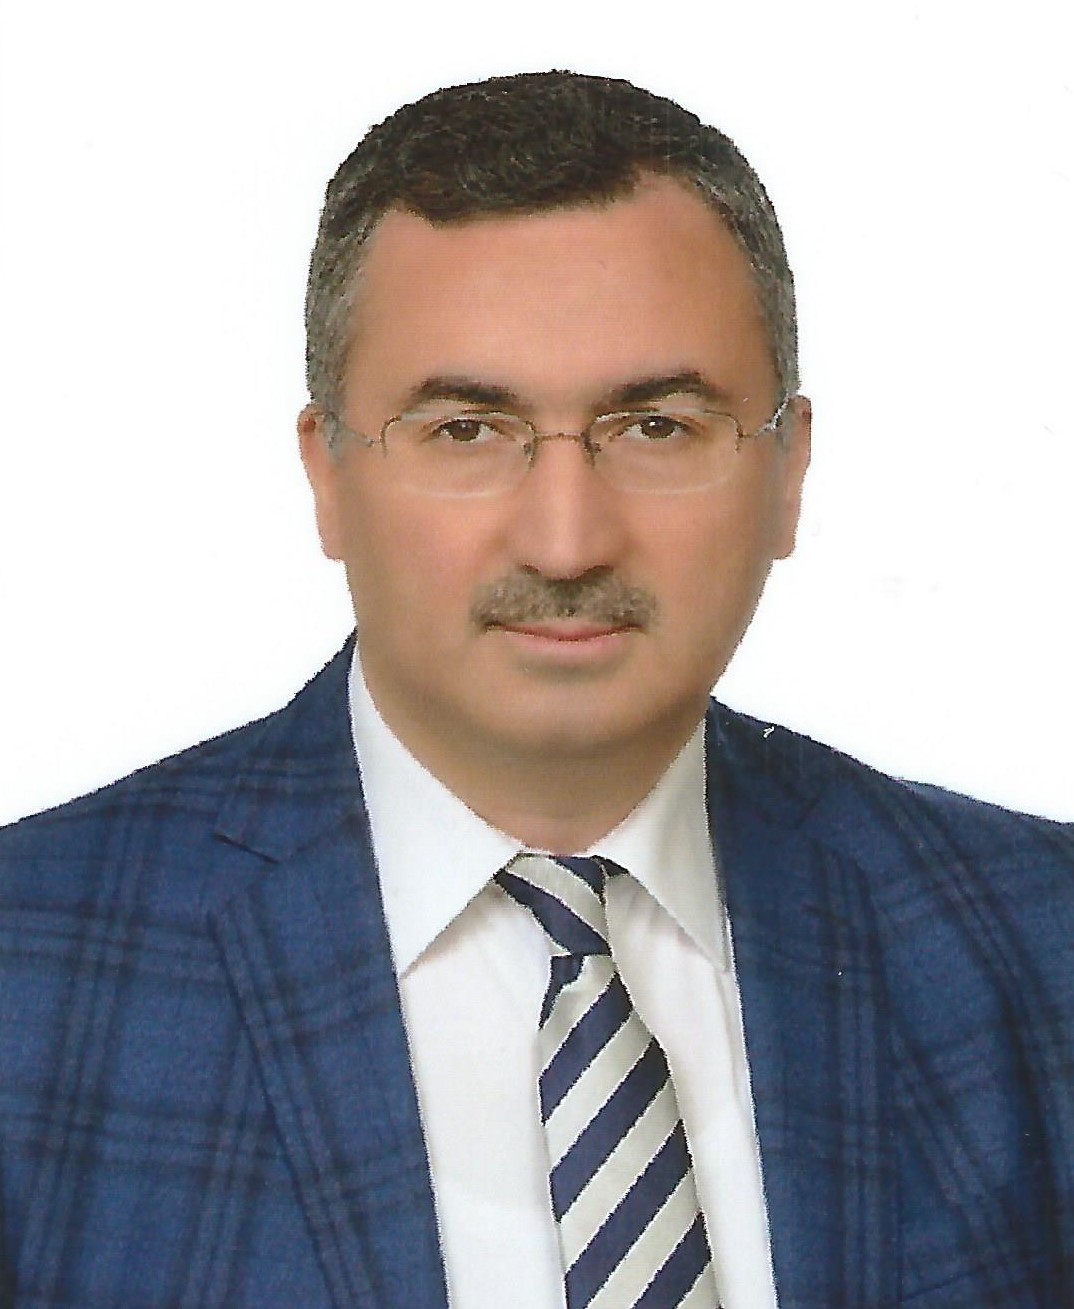
\includegraphics[width=1in,height=1.25in,clip,keepaspectratio]{figures/foto_ahmet.jpg}}]{Ahmet Altuncu}
    received the Ph.D. degree in electronic systems engineering from the University of Essex, Colchester, U.K., in 1998. He founded and directed the Photonics Technologies Application and Research Center at Dumlupinar University. He is currently a Professor with the Department of Electrical and Electronics Engineering, Afyon Kocatepe University, Afyonkarahisar, Turkiye. His research interests include doped-fiber optical amplifiers, CW and pulsed fiber lasers, and optical sensors. He is the author of more than 50 international journal and conference papers.
\end{IEEEbiography}

\begin{IEEEbiography}[{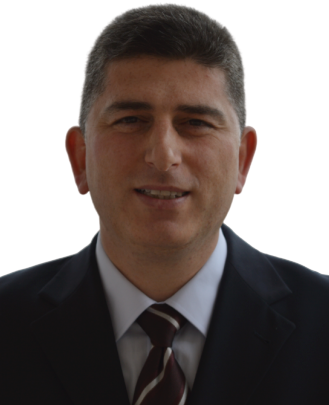
\includegraphics[width=1in,height=1.25in,clip,keepaspectratio]{figures/foto_mustafa.jpg}}]{Mustafa Namdar}
    (Member, IEEE) received the B.Sc. and Ph.D. degrees in electronics and communications engineering from Yildiz Technical University, Istanbul, Turkiye. From 2000 to 2011, he was with Turkcell, Istanbul, Turkiye, where he participated in several wireless communications projects. He is currently an Associate Professor with the Department of Electrical and Electronics Engineering, Kutahya Dumlupinar University, Kutahya, Turkiye. His research interests include cognitive radio networks, interference alignment, nonorthogonal multiple access (NOMA), reconfigurable intelligent surfaces (RIS), and integrated sensing and communication (ISAC).
\end{IEEEbiography}
